\subsection{Analisi}
\label{analisi}
\textbf{Durata:} dal 2020\_11\_06 al 2021\_01\_11\\
Durante questo periodo si forma il gruppo che si prepara alla \glo{\textbf{RR}}, studiando i \glo{capitolati} proposti e svolgendo un'analisi preliminare dei requisiti e la pianificazione globale del lavoro da svolgere. 
Le precondizioni sono:
\begin{itemize}
    \item Formazione del gruppo;
    \item Presentazione dei \glo{capitolati}.
\end{itemize}
Le postcondizioni sono:
\begin{itemize}
    \item Scelta del nome e del logo del gruppo;
    \item Creazione della mail e di un \glo{repository} \glo{GitHub};
    \item Scelta del capitolato;
    \item Redazione dei documenti quali: {\SdF}, {\NdP}, {\PdP}, {\Glossario}, \textit{Lettera di presentazione}, {\PdQ}, {\AdR} ed i verbali;
    \item Verifica e approvazione di quanto redatto.
\end{itemize}
Questa periodo è composto da sette attività che corrispondono ai documenti prodotti:
\begin{itemize}
    \item \textbf{Studio di fattibilità:} Vengono analizzati i vari capitolati per evidenziarne gli aspetti negativi e positivi. Dopo un periodo di studio e confronto {\Gruppo} dà la preferenza in quello più adatto. L'attività è bloccante per l'{\AdR};
    \item \textbf{Norme di progetto:} Vengono definite tutte le regole che il gruppo {\Gruppo} dovrà seguire per la stesura dei documenti e per lo sviluppo del progetto;
    \item \textbf{Glossario:} Contiene tutti i termini che possono risultare ambigui durante lo svolgimento del progetto; di essi viene fornita una definizione sintetica ed esaustiva;
    \item \textbf{Lettera di presentazione:} Documento in cui il gruppo {\Gruppo} si candida al capitolato scelto come fornitore del prodotto software richiesto;
    \item \textbf{Piano di progetto:} Nel presente documento sono descritte le attività, i rischi del progetto e viene calcolato il preventivo per la realizzazione di progetto. Presenta poi la suddivisione del lavoro tra i membri del gruppo {\Gruppo} e il calcolo del preventivo;
    \item \textbf{Analisi dei requisiti:} Vengono studiati e analizzati nel dettaglio i requisiti del capitolato scelto nello {\SdF};
    \item \textbf{Piano di qualifica:} Si individuano metodi e procedure per garantire la \glo{qualità} del prodotto.
\end{itemize}
La pianificazione di questo periodo è stata organizzata nel modo seguente:
\begin{enumerate}
\item \textbf{2020\_11\_06 - 2020\_12\_03}:
Inizio della stesura delle {\NdP} per avere delle regole condivise dal gruppo per svolgere il lavoro. Durante la stesura di queste, il gruppo si confronta riguardo ai vari capitolati esponendo le preferenze personali di ciascun componente del gruppo. Viene analizzato ogni capitolato focalizzando l'attenzione principalmente verso i loro aspetti positivi e negativi e dei possibili rischi che si possono incontrare per ognuno. Dopo i confronti iniziali si è potuto iniziare uno studio sulla fattibilità generico per tutti i capitolati per poi approfondirlo per i capitolati che suscitavano più interesse al gruppo e iniziare a stilare il {\Glossario} per la registrazione dei termini, usati nei documenti, che potrebbero creare ambiguità. Durante questo periodo sono state prese decisioni tecniche e organizzative come: nome del gruppo, logo, indirizzo mail, creazione \glo{repository} e i vari mezzi di comunicazione. Vengono trascritti i verbali interni relativi alle riunioni del gruppo durante questo arco di tempo;
\item \textbf{2020\_12\_04 - 2020\_12\_21}:
Inizio della stesura del {\PdP}, contenente la pianificazione del lavoro da svolgere e la suddivisione dei ruoli tra i membri del gruppo. Stesa una prima bozza della \textit{Lettera di presentazione}, il cui completamento sarà fatto dopo la conclusione del {\PdP} con l'aggiunta del prospetto economico finale. Integrato il {\Glossario} quando necessario. In data 2020\_12\_22 il gruppo ha fissato una \glo{milestone} per il completamento dei documenti iniziati durante questo periodo, ad eccezione dell'ultima sezione del {\PdP} destinata al consuntivo finale del periodo successivo. Iniziano le attività di verifica incrementale per i documenti in corso di stesura. Stesi i verbali interni relativi agli incontri svolti;
\item \textbf{2020\_12\_22 - 2021\_01\_07}:
Inizio della stesura dell'{\AdR} e del {\PdQ}, con l'esposizione dei criteri di valutazione della qualità scelti dal gruppo e le rispettive metriche di calcolo. Continuano le attività di verifica incrementale per i documenti in corso di stesura;
\item \textbf{2021\_01\_08 - 2021\_01\_11}
Il gruppo svolge le ultime attività di verifica sugli ultimi documenti, completa il {\Glossario} e uniforma tutti i prodotti alle regole stabilite nelle {\NdP} se necessario.
\end{enumerate}
\subsubsection{Diagramma di Gantt: Analisi}
\begin{figure}[ht]
    \centering
    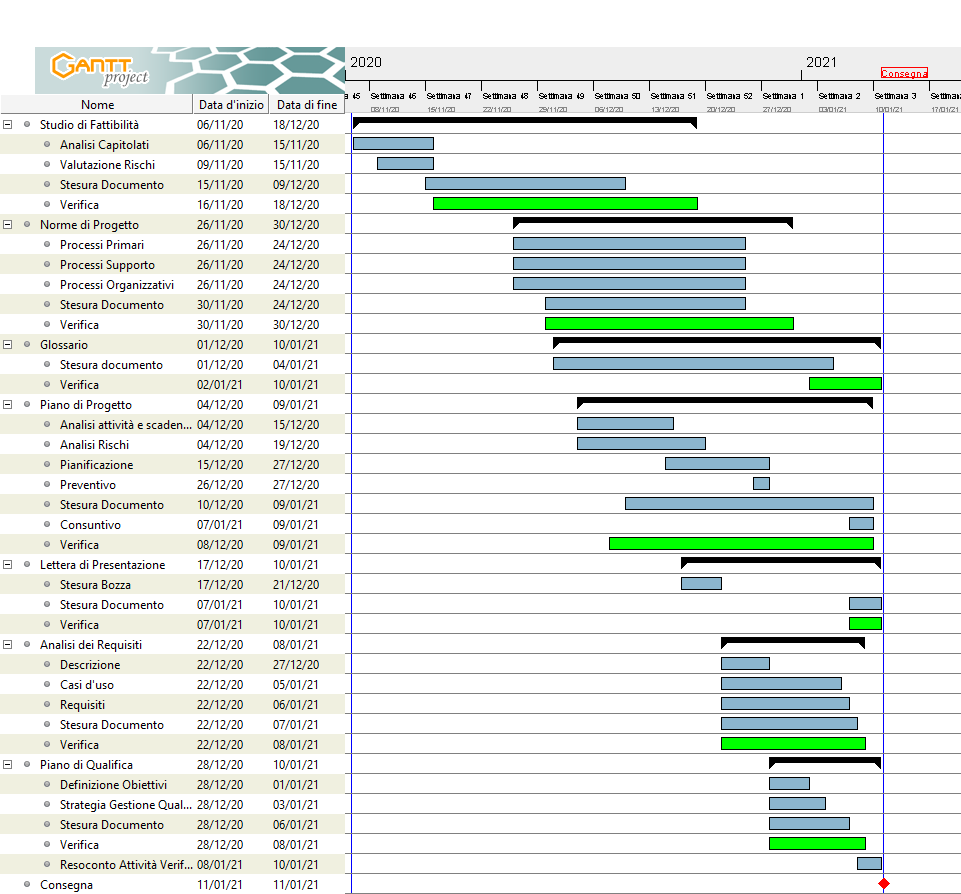
\includegraphics[width=\textwidth]{Immagini/GanttAnalisi}
    \caption{Diagramma di Gantt dell'attività di analisi}
\end{figure}